%%% Для сборки выполнить 2 раза команду: pdflatex <имя файла>

\documentclass[a4paper,12pt]{article}

\usepackage{ucs}
\usepackage[utf8x]{inputenc}
\usepackage[russian]{babel}
%\usepackage{cmlgc}
\usepackage{graphicx}
\graphicspath{ {./images/} }
\usepackage{listings}
\usepackage{xcolor}
\usepackage{hyperref}
\hypersetup{
    colorlinks=true,
    linkcolor=black,
    filecolor=black,      
    urlcolor=cyan,
    pdftitle={НИР},
    pdfpagemode=FullScreen,
    }
\usepackage{float}
%\usepackage{courier}


% для поддержки джаваскрипта. сурс - tex.stackexchange.com %
\usepackage{color}
\definecolor{lightgray}{rgb}{.95,.95,.95}
\definecolor{darkgray}{rgb}{.4,.4,.4}
\definecolor{purple}{rgb}{0.53, 0.26, 0.75}
\definecolor{maroon}{rgb}{0.7, 0.24, 0.2}
\definecolor{cobalt}{rgb}{0.03, 0.44, 0.73}
\lstdefinelanguage{JavaScript}{
  keywords={break, case, catch, continue, debugger, default, delete, do, else, false, finally, for, function, if, in, instanceof, new, null, return, switch, this, throw, true, try, typeof, var, void, while, with},
  morecomment=[l]{//},
  morecomment=[s]{/*}{*/},
  morestring=[b]',
  morestring=[b]",
  ndkeywords={class, export, boolean, throw, implements, import, this},
  keywordstyle=\color{cobalt}\bfseries,
  ndkeywordstyle=\color{darkgray}\bfseries,
  identifierstyle=\color{black},
  commentstyle=\color{purple}\ttfamily,
  stringstyle=\color{maroon}\ttfamily,
  sensitive=true
}

\lstset{
   language=JavaScript,
   backgroundcolor=\color{lightgray},
   extendedchars=true,
   basicstyle=\footnotesize\ttfamily,
   showstringspaces=false,
   showspaces=false,
   numbers=left,
   numberstyle=\footnotesize,
   numbersep=9pt,
   tabsize=2,
   breaklines=true,
   showtabs=false,
   captionpos=b
}

\makeatletter
\renewcommand\@biblabel[1]{#1.}
\makeatother

\newcommand{\myrule}[1]{\rule{#1}{0.4pt}}
\newcommand{\sign}[2][~]{{\small\myrule{#2}\\[-0.7em]\makebox[#2]{\it #1}}}

% Поля
\usepackage[top=20mm, left=30mm, right=10mm, bottom=20mm, nohead]{geometry}
\usepackage{indentfirst}

% Межстрочный интервал
\renewcommand{\baselinestretch}{1.50}


\begin{document}

%%%%%%%%%%%%%%%%%%%%%%%%%
%%%                   %%%
%%% Титульный лист    %%%

\thispagestyle{empty}
\begin{center}


\renewcommand{\baselinestretch}{1}
{\large
{\sc Петрозаводский государственный университет\\
Институт математики и информационных технологий\\
	Кафедра Информатики и Математического Обеспечения
}
}

\end{center}


\vfill

\begin{center}
{\normalsize Отчет о научно-исследовательской работе} \\

\medskip

%%% Название работы %%%
	{\Large \sc Разработка клиентской части веб-сервиса для коллективных переводов} \\
\end{center}

\medskip

\begin{flushright}
\parbox{11cm}{%
\renewcommand{\baselinestretch}{1.2}
\normalsize
	Выполнила:\\
студентка 3 курса группы 22305
\begin{flushright}
	 С. Э. Зименкова \sign[подпись]{4cm}
\end{flushright}




Научный руководитель:\\
%%% степень, звание ФИО научного руководителя %%%
% Первый руководитель 
Д. Б. Чистяков \\
\begin{flushright}
\sign[подпись]{4cm}
\end{flushright}

Итоговая оценка \\
\begin{flushright}
\sign[оценка]{4cm}
\end{flushright}

% Второй руководитель 
% И. О. Фамилия, ученая степень, ученое звание \\
% \begin{flushright}
% \sign[подпись]{4cm}
% \end{flushright}
}
\end{flushright}

\vfill

\begin{center}
\large
    Петрозаводск --- 2024
\end{center}

%%% Титульный лист    %%%
%%%                   %%%
%%%%%%%%%%%%%%%%%%%%%%%%%


%%%%%%%%%%%%%%%%%%%%%%%%%
%%%                   %%%
%%% Содержание        %%%

\newpage

\tableofcontents

%%% Содержание        %%%
%%%                   %%%
%%%%%%%%%%%%%%%%%%%%%%%%%


%%%%%%%%%%%%%%%%%%%%%%%%%
%%%                   %%%
%%% Введение          %%%

\newpage
\section*{Введение}
\addcontentsline{toc}{section}{Введение}

Перевод больших массивов текста зачастую является трудоемкой задачей, требующей большого количества времени. Задача усложняется, если необходимо перевести художественное произведение, научную работу, текст выступления на конференции или справочные материалы, содержащие большое количество специальной лексики. Процесс перевода становится более эффективным, если он выполняется коллективом профессионалов, выполняющих разные роли: помимо самих переводчиков в работе принимают участие редакторы и руководители проекта, которым нужно разделять обязанности между работниками, согласовывать процесс и утверждать прошедшие редакцию главы. \\

Профессиональный перевод не является единственной возможной формой работы над текстом на иностранном языке. Не все заказчики могут позволить себе оплатить профессиональный перевод значительного по объему текста. Примером подобных текстов могут выступать интерфейс ПО и компьютерных игр, узконаправленная литература, конспекты лекций и конференций, субтитры к видеоматериалам, находящимся в открытом доступе. Такую работу часто выполняют волонтеры, не все из которых обладают достаточными навыками для выполнения профессионального перевода. В проектах, связанных с любительским переводом, помимо синхронизации и распределения частей текста между участниками, необходимо проверять качество работы и выбирать наилучшие варианты перевода, так как волонтеры и любители не несут достаточной ответственности за свою работу и не могут гарантировать его верность. \\

Решением проблемы распределения, синхронизации и утверждения перевода для команд переводчиков любой степени профессионализма является удобный инструмент, позволяющий пользователям совместно работать над переводом.\\

Разработка веб-сервиса разделена на три этапа:
\begin{itemize}
	\item разработка структуры (веб-API, база данных) и веб-страниц;
	\item установка связи между back-end и front-end составляющими проекта, разработка инструмента-редактора;
	\item доработка и улучшение сервиса, расширение функционала.\\
\end{itemize}

Цель данной работы — разработать клиентскую часть веб-сервиса для коллективных переводов. На предыдущем этапе уже были реализованы HTML-шаблоны с подключенными стилями, поэтому на этом этапе необходимо внести улучшения в существующие шаблоны, сделать их динамическими и осуществить взаимодействие клиентской части с веб-API.

Для осуществления поставленной цели необходимо выполнить следующие задачи:
\begin{itemize}
	\item Сформулировать требования к клиентской части веб-сервиса;
	\item Доработать макет пользовательского интерфейса;
	\item Разработать и интегрировать клиентскую часть веб-сервиса в информационную систему.
\end{itemize}

%%% Введение          %%%
%%%                   %%%
%%%%%%%%%%%%%%%%%%%%%%%%%



%%%%%%%%%%%%%%%%%%%%%%%%%
%%%                   %%%
%%% Глава 1           %%%

\newpage
\section{Анализ предметной области}
\subsection{Описание требований к разрабатываемому сервису}

Разрабатываемый сервис для удобства получил временное название "Desman Translate".\\

\subsubsection{Глоссарий}
\begin{itemize}
\item \textbf{Текст} — содержание книг, субтитров, подписей в компьютерных программах и др.
\item \textbf{Раздел} — набор отрывков текста, объединенных в массив по усмотрению пользователя для его удобства.
\item \textbf{Участник} — пользователь, имеющий доступ к работе над текстом в проекте.
\end{itemize}

\subsubsection{Описание функционала разрабатываемого сервиса}
\textbf{Desman Translate} — веб-сервис, позволяющий пользователям совместно работать над проектами по переводу текстов. Сервис реализован в виде веб-сайта.\\

Сервис рассчитан на два типа переводчиков:
\begin{itemize}
\item Переводчики-любители, которым нужно найти команду, т. к. они не могут перевести некоторое произведение в одиночку. Для удобства таких пользователей сервис должен предоставлять возможность для работы большого количества людей над одним и тем же текстом, а также поиска существующих проектов, где пользователи могли бы предоставить помощь с переводом, и популяризации своих проектов, чтобы найти других переводчиков, которые готовы помочь.
\item Переводчики-профессионалы, которым нужен инструмент для совместной асинхронной работы над переводом, а также возможность распределения работы между членами команды, рецензирования готового перевода. Профессиональным командам также важна возможность скрыть свою работу от публики и не допустить других людей до работы над текстом, т. к. они могут работать над произведением или программой, защищенными авторским правом.
\end{itemize}

\textbf{Проект} — это созданная пользователем страница сайта, которая определяет процесс работы над некоторым произведением. Проект имеет название, описание, раздел, участников, статус (в работе, заморожен, закрыт), видимость (открытый, скрытый). Статус проекта влияет на представление и доступ к работе над текстом. Замороженный проект — незавершенный перевод, над которым временно прекращена работа; участники не могут работать с текстом, пока владелец проекта не откроет его вновь. Закрытый проект — завершенный перевод, в котором больше нельзя загружать разделы и работать над текстом. Проект также может быть публичным и приватным. Эта возможность добавлена для того, чтобы проект мог отображаться или не отображаться в поиске и быть видимым для пользователей, не являющихся участниками. Владелец проекта может скрыть свой проект от других пользователей по своему усмотрению (например, если переводимый текст защищен авторским правом и не должен быть в открытом доступе). Для проекта можно настроить и другие параметры. Например, для каждого типа пользователей можно отдельно настроить права доступа к проекту (например, могут ли пользователи, не являющиеся участниками, читать текст, загруженный в проект; могут ли пользователи присоединяться к проекту без приглашения/одобрения).\\

Работа над переводом осуществляется следующим образом:

\begin{itemize}
\item Пользователь, имеющий соответствующие права доступа, загружает в проект текст.
\item Текст автоматически или по усмотрению пользователя разбивается на отрывки. Отрывком может быть строка, абзац, страница и любое другое количество текста.
\item Пользователи могут добавлять для отрывков свои варианты перевода и голосовать за лучший вариант.
\item Лучший по результатам голосования вариант перевода отображается вверху списка и считается итоговым переводом.
\item Варианты переводов объединяются в текст при экспорте перевода. Пользователь может скачать переведенный текст и использовать его далее по своему усмотрению. Пользователь может экспортировать объединение лучших вариантов перевода или объединение вариантов перевода от отдельного пользователя. Таким образом может быть получен лучший текст по результатам голосования, а также несколько переводов от разных переводчиков.
\end{itemize}

Есть несколько типов пользователей: незарегистрированный пользователь и зарегистрированный пользователь. Незарегистрированный пользователь может зарегистрироваться или войти в аккаунт, просматривать существующие проекты на сайте.\\

Зарегистрированный пользователь может иметь разные роли в разных проектах. Зарегистрированный пользователь может просматривать существующие проекты, присоединяться к существующим проектам, создавать свои проекты (становясь при этом владельцем созданного проекта), модерировать свои проекты (в том числе назначать роли участников проекта), загружать тексты, разбивать тексты на разделы и отрывки, работать над переводом отрывков. Участник проекта может иметь следующие роли в проекте:
\begin{itemize}
\item Переводчик имеет возможность добавлять варианты перевода отрывков, голосовать за лучший вариант перевода.
\item Редактор может все, что может переводчик, а также может редактировать существующие варианты перевода и имеет больший вес голоса при выборе лучшего варианта \item перевода.
\item Модератор может все, что может переводчик, а также может назначать роли пользователей (исключение: не может понизить роль владельца и других модераторов), редактировать информацию о проекте, приглашать пользователей стать участниками проекта.
\item Владелец может все, что могут редактор и модератор, но также может загружать и удалять разделы, понижать роли модераторов, менять права доступа к проекту, менять видимость проекта, менять статус проекта и другие параметры.
\item Все перечисленные роли могут быть настроены владельцем, а отдельному пользователю можно выдать дополнительные права. Пользователь может иметь несколько ролей одновременно (например, быть и редактором, и модератором).
\end{itemize}

Зарегистрированный пользователь может подать заявку на присоединение к публичному проекту. Владелец и модераторы проекта могут одобрить или отклонить заявку; если заявка была одобрена, пользователь становится участником проекта. Владелец и модераторы проекта могут пригласить пользователя в проект. Пользователь может принять или отклонить приглашение; если пользователь принял приглашение, он становится участником проекта.

Сервис также предоставляет доступ для удобного поиска существующих проектов. Для этого проектам присваиваются такие параметры как язык оригинала, язык перевода, тип (книга, субтитры, программа...), жанр (жанры книг, жанры фильмов и сериалов, типы программ) и популярность (например, количество посещений). Сервис имеет раздел поиска проектов, в котором пользователь может фильтровать проекты по названным параметрам или искать по названию на языке оригинала и языке перевода.

Пользователь также имеет свою собственную страницу на сайте. На этой странице пользователь может указать информацию о себе (например, уровень знания языков и область знаний/интересов), аватар (изображение, отображаемое рядом с именем пользователя), настроить свои контактные данные, имя пользователя и пароль, менять параметры пользователя, удалить свой аккаунт. Другие пользователи видят на странице этого пользователя информацию, которая поможет им выбрать приглашаемого переводчика или определить, стоит ли одобрить его заявку на вступление. Эта информация содержит имя пользователя, его аватар, его описание себя и проекты, в которых этот пользователь участвует.

\subsubsection{Требования к разделам, доступным пользователям на сайте}

\begin{enumerate}
\item Панель навигации
\begin{enumerate}
	\item Панель навигации должна быть доступна в шапке каждой страницы веб-сервиса, кроме текстового редактора.
	\item Панель навигации предоставляет пользователю возможность переходить на следующие страницы: Главная страница, Список проектов пользователя, Личный кабинет, Поиск проектов, Авторизация, Регистрация.
\end{enumerate}
\item Список проектов пользователя
\begin{enumerate}
	\item Список проектов пользователя предоставляет пользователю список проектов, в которых он является участником или владельцем, краткую информацию о них и роль пользователя в этом проекте.
	\item Список проектов пользователя должен позволять пользователю перейти на страницу выбранного проекта.
	\item Со страницы списка проектов можно перейти на страницу создания проекта.
	\item На странице списка проектов пользователя есть список приглашений в проекты, которые пользователь может принять или отклонить.
\end{enumerate}
\item Страница регистрации
\begin{enumerate}
	\item Пользователь вводит электронную почту, логин и пароль. При нажатии на кнопку "Зарегистрироваться" создается новая учетная запись.
\end{enumerate}
\item Страница авторизации
\begin{enumerate}
	\item Пользователь вводит логин, пароль и авторизуется.
	\item Пользователь может сменить пароль, если он его забыл.
\end{enumerate}
\item Главная страница
\begin{enumerate}
	\item Главная страница должна предоставлять возможность пользователю сервиса видеть свои последние проекты и ведущиеся на данный момент популярные переводы.
	\item Главная страница должна предоставлять возможность осуществлять быстрый поиск проектов по названию или ID.
	\item Главная страница должна предоставлять новому пользователю возможность получить информацию о веб-сервисе.
	\item С главной страницы можно перейти на страницу создания проекта.
\end{enumerate}
\item Личный кабинет
\begin{enumerate}
	\item Личный кабинет должен предоставлять возможность пользователю редактировать информацию о своём профиле, такую как отображаемое имя (nickname), аватар и информацию о себе.
	\item Личный кабинет должен предоставлять возможность пользователю редактировать для себя настройки интерфейса сервиса (внешний вид сайта).
	\item Личный кабинет должен предоставлять возможность пользователю изменять и восстанавливать пароль от аккаунта в случае потери.
	\item В личном кабинете указаны все проекты, в которых участвует пользователь.
	\item Из личного кабинета можно перейти на страницу создания проекта.
\end{enumerate}
\item Страница проекта
\begin{enumerate}
	\item На странице проекта для удобства содержимое разделено на вкладки.
	\item На вкладке "Проект" пользователю должна быть доступна информацию о проекте: название, обложка, описание, список разделов.
	\item На вкладке "Проект" владелец проекта может загружать разделы при помощи файлов, в т. ч. с различным форматированием, таким как JSON или CSV.
	\item На вкладке "Проект" пользователь, не являющийся участником, может нажать на кнопку "Присоединиться к проекту".
	\item На вкладке "Проект" участник проекта может зайти в редактор отрывков.
	\item На вкладке "Участники" участникам проекта доступен список участников, модераторы и владелец могут удалять и приглашать участников.
	\item На вкладке "Настройки" модераторы и владелец проекта могут менять информацию о проекте, владелец может удалить свой проект.
\end{enumerate}
\item Меню управления проектом
\begin{enumerate}
	\item Модератор должен иметь возможность изменять такие редактируемые данные как информация о проекте, название, обложка, разделы проекта, участники проекта, язык оригинала, язык перевода и параметры проекта.
	\item Меню проекта должно предоставлять возможность имеющим права участникам скачивать полученный перевод в запрашиваемом формате (JSON, CSV...) и с заданными фильтрами (лучший перевод, перевод конкретного пользователя).
	\item Меню проекта должно предоставлять возможность имеющим права участникам приглашать новых пользователей участвовать в данном проекте.
	\item Модератор может менять роли участников.
\end{enumerate}
\item Текстовый редактор
\begin{enumerate}
	\item Текстовый редактор должен предоставлять возможность переводчику добавлять новые переводы данных в разделе отрывки.
	\item Текстовый редактор должен предоставлять возможность пользователю-редактору изменять и удалять отрывки других участников.
	\item Участник проекта может голосовать за отрывки других участников.
\end{enumerate}
\item Поиск проектов
\begin{enumerate}
	\item Поиск проектов должен позволять фильтровать проекты по тем или иным признакам (популярность, жанр, язык оригинала и перевода), а также выделять отдельно доступные для вступления проекты.
	\item Поиск проектов должен предоставлять возможность найти нужный проект по названию или ID.
\end{enumerate}
\item Страница создания проектов
\begin{enumerate}
	\item Страница создания проектов должна позволять пользователю создать новый проект.
	\item Пользователь должен иметь возможность указать следующую информацию о проекте: Название проекта, Уникальная ссылка, Язык оригинала, Язык перевода, Обложка проекта, Доступ к проекту.
\end{enumerate}
\end{enumerate}

\subsubsection{Модели требований}
\paragraph{Модель предметной области}
\subparagraph{Объекты предметной области}
\begin{itemize}
\item Неавторизованный пользователь — посетитель сайта, не прошедший этап авторизации.
\item Авторизованный пользователь — посетитель сайта, прошедший регистрацию.
\item Главная страница — страница сайта, которая содержит недавние и популярные проекты.
\item Проект — совокупность пользователей, участвующих в переводе некоторого произведения, и набора отрывков текста, которые относятся к этому произведению.
\item Участник — пользователь, имеющий доступ к работе над текстом в проекте.
\item Текст — содержимое для перевода, загружается на страницу проекта.
\item Отрывок — небольшая часть текста, доступная для перевода по отдельности.
\item Свойства и информация о проекте — параметры проекта, которые может просмотреть любой пользователь, редактируются владельцем.
\item Вариант перевода — относятся к отрывкам, за них можно голосовать и редактировать в соответствии с ролью.
\item Популярные проекты — проекты с самым большим количеством просмотров.
\item Недавние проекты — проекты, упорядоченные по дате создания, начиная с новых.
\item Модуль регистрации — модуль, отвечающий за создание новых учетных записей для неавторизованных пользователей.
\item Модуль авторизации — модуль, дающий неавторизованным пользователям возможность войти в свою учетную запись.
\item Окно смены пароля — модуль, позволяющий восстановить пароль пользователю.
\item Личный кабинет — страница с информацией о пользователе: имя, логин, описание, а также все проекты, в которых он участвует.
\item Настройки интерфейса — смена цвета темы, шрифта.
\item Роль проекта: переводчик — имеет возможность добавлять варианты перевода отрывков, голосовать за лучший вариант перевода.
\item Роль проекта: редактор — может редактировать существующие варианты перевода и имеет больший вес голоса при выборе лучшего варианта перевода.
\item Роль проекта: модератор — может назначать роли пользователей (исключение: не может понизить роль владельца и других модераторов), редактировать информацию о проекте, приглашать пользователей стать участниками проекта.
\item Роль проекта: владелец — может загружать и удалять разделы, понижать роли модераторов, менять права доступа к проекту, менять видимость проекта, менять статус проекта и другие параметры.
\end{itemize}

Далее представлены диаграммы процессов предметной области: навигация по веб-сайту и структура проекта.\\

\begin{figure}[H]
\centering
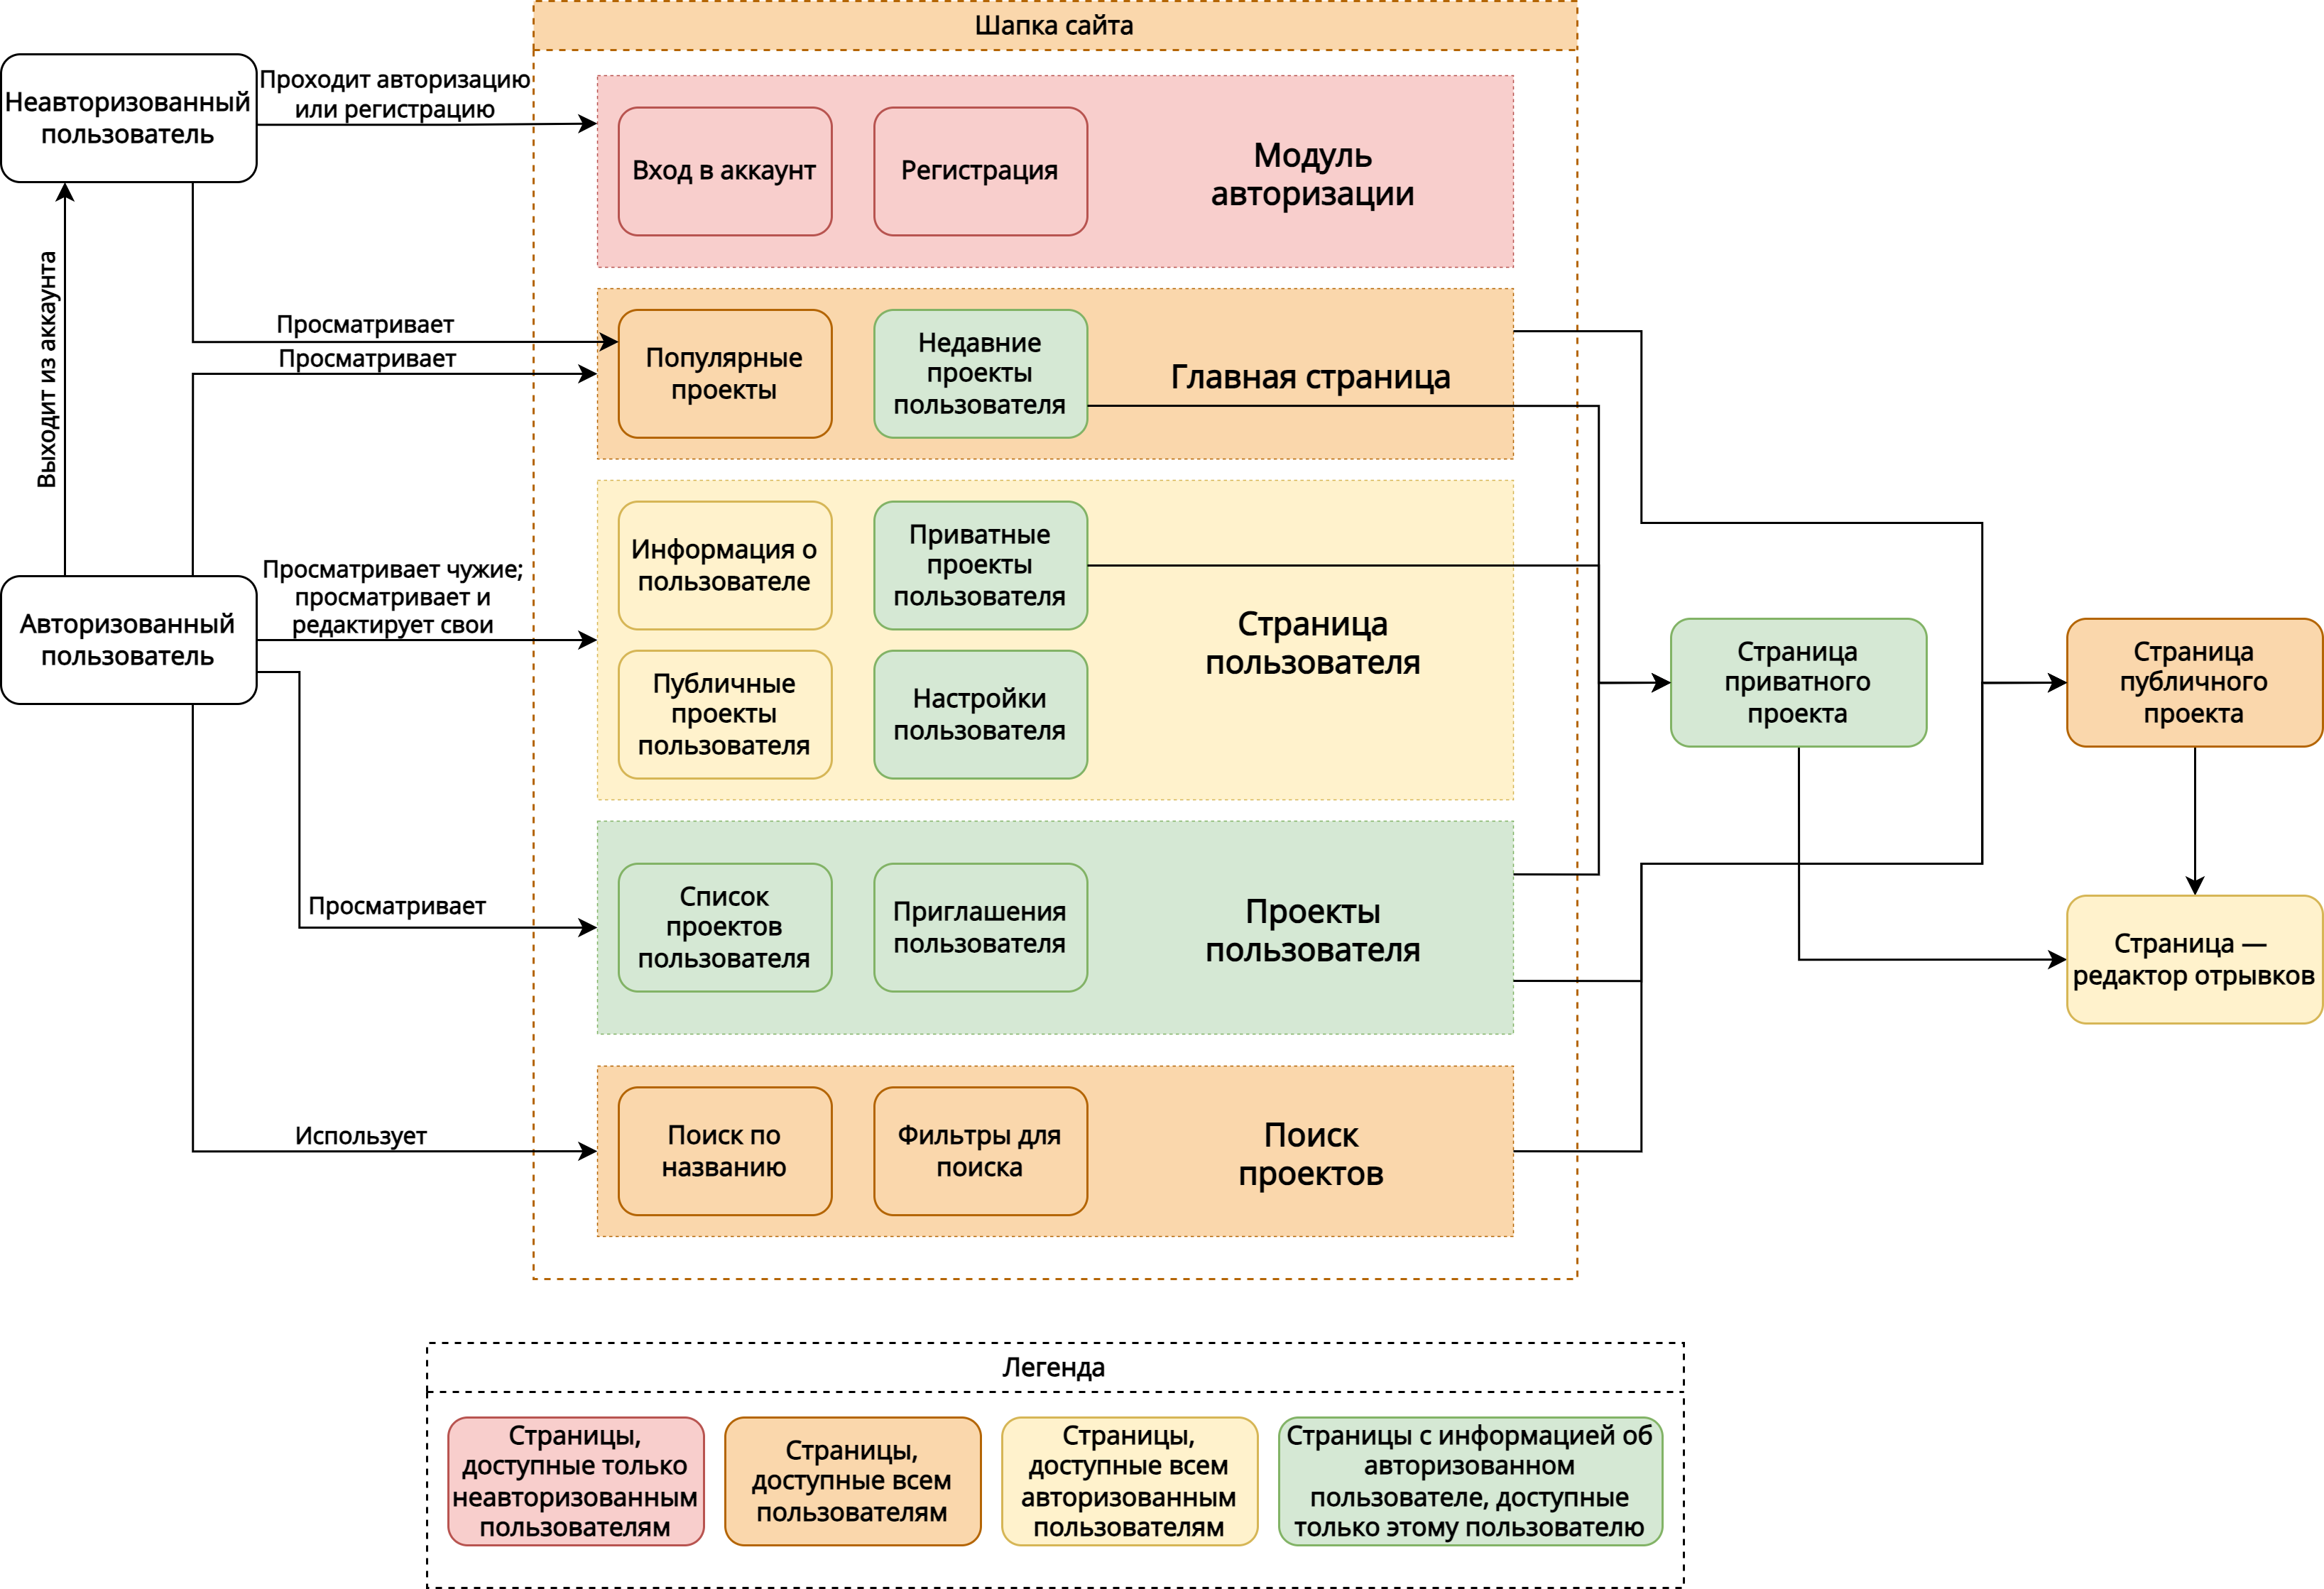
\includegraphics[width=\textwidth]{/diagrams/PagesDiagram.png}
\caption{Диаграмма процессов предметной области: навигация по веб-сайту.}
\label{fig:diagrampages}
\end{figure}

\begin{figure}[H]
\centering
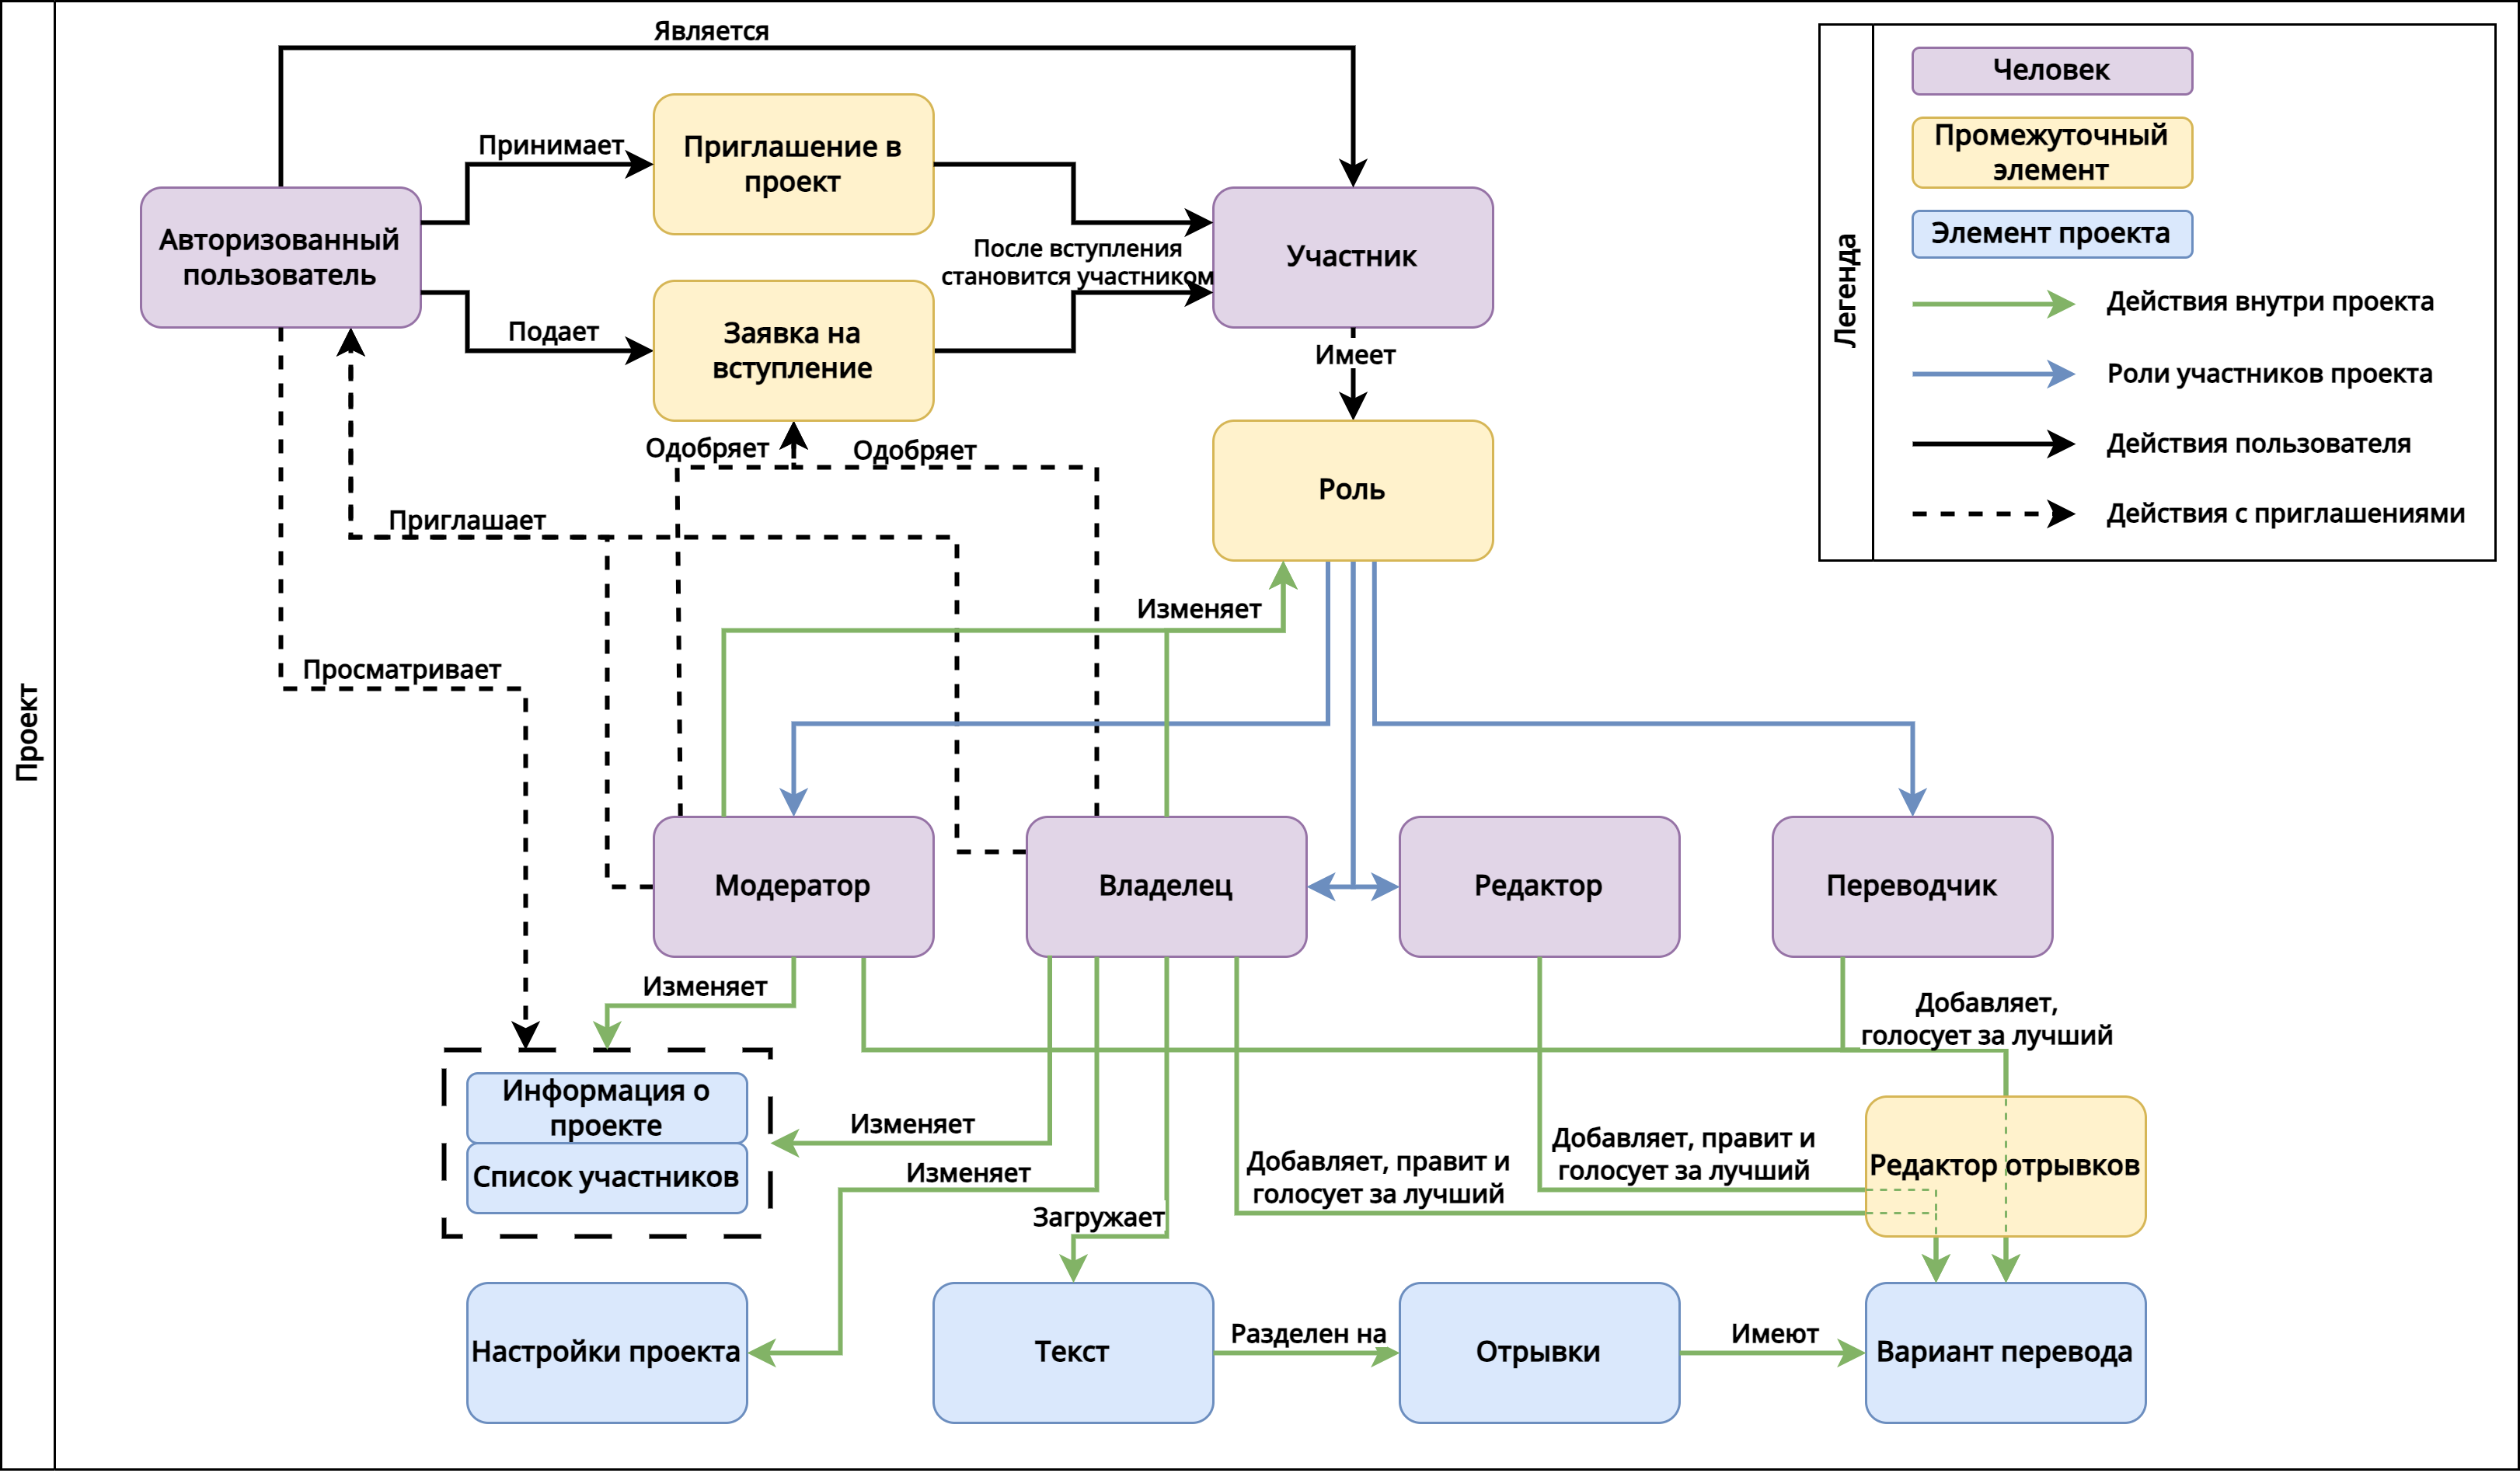
\includegraphics[width=\textwidth]{/diagrams/ProjectDiagram.png}
\caption{Диаграмма процессов предметной области: структура проекта.}
\label{fig:diagramproject}
\end{figure}

\paragraph{Модель предметной области}
\subparagraph{Список пользователей}
\begin{itemize}
\item Неавторизованный пользователь.
\item Авторизованный пользователь.
\end{itemize}

\subparagraph{Права пользователей}
\begin{itemize}
\item Все пользователи:

\begin{itemize}
\item Посетить главную страницу.
\item Увидеть популярные проекты.
\end{itemize}

\item Неавторизованный пользователь:

\begin{itemize}
\item Пройти регистрацию в окне регистрации, чтобы создать новую учетную запись.
\item Войти в существующую учетную запись.
\end{itemize}

\item Авторизованный пользователь:

\begin{itemize}
\item Выйти из учетной записи.
\item Войти в личный кабинет:
	\begin{itemize}
	\item Перейти на окно смены пароля.
	\item Увидеть информацию о пользователе.
	\item Увидеть проекты, в которых он участвует.
	\end{itemize}
\item Создать новый проект.
\item Зайти в один из проектов, в котором он участвует.
	\begin{itemize}
	\item Увидеть участников проекта.
	\item Увидеть процесс выполнения проекта.
	\item Увидеть информацию о проекте.
	\item Увидеть описание проекта.
	\item Выполнять действия в соответствии с ролью в проекте.
	\end{itemize}
\item Увидеть публичные проекты.
\item Осуществить поиск по названию проекта.
\item Написать разработчику.
\end{itemize}
\end{itemize}

\subparagraph{Интересы пользователя}

\begin{itemize}
\item Неавторизованный пользователь:
\begin{itemize}
\item Доступная информация о назначении сайта и его использовании другими пользователями.
\item Информирование о необходимости в авторизации.
\item Удобный интерфейс для авторизации и регистрации.
\end{itemize}

\item Авторизованный пользователь:
\begin{itemize}
\item Удобные средства для поиска, создания проектов, возможности к ним присоединиться.
\item Удобные средства для работы в проекте (см. модель участников проекта).
\end{itemize}
\end{itemize}

\paragraph{Модель участников проекта}

\begin{itemize}
\item Авторизованные пользователи, присоединившиеся к проекту, получают одну из ролей проекта. Все участники проекта имеют права переводчика, отличная от переводчика роль добавляет участнику другие права.
\end{itemize}

\textbf{Список ролей}

\begin{itemize}
\item Переводчик
\item Редактор
\item Модератор
\item Владелец
\end{itemize}


\textbf{Права роли}\\

Переводчик:

\begin{itemize}
\item Может добавлять и редактировать свои варианты перевода отрывков.
\item Может голосовать за лучший вариант отрывка.
\end{itemize}

Редактор:

\begin{itemize}
\item Имеет все права переводчика.
\item Может редактировать чужие варианты перевода.
\end{itemize}

Модератор:

\begin{itemize}
\item Имеет все права переводчика.
\item Может назначать роли участников (не может изменить роли модераторов и владельца).
\item Может приглашать новых участников, одобрять заявки на вступление в проект.
\item Может редактировать информацию о проекте.
\end{itemize}

Владелец:

\begin{itemize}
\item Имеет все права переводчика, редактора и модератора.
\item Может создавать и удалять разделы.
\item Может изменять роли модераторов.
\item Может менять статус проекта и его видимость.
\end{itemize}


\textbf{Интересы роли}\\

Переводчик:
\begin{itemize}
\item Удобный интерфейс для просмотра текста и вариантов перевода.
\item Простая система для голосования за лучший перевод.
\item Простой и удобный интерфейс для добавления вариантов перевода.
\end{itemize}

Редактор:
\begin{itemize}
\item Интересы роли переводчика.
\item Простой и удобный интерфейс для добавления и изменения вариантов перевода.
\end{itemize}

Модератор:

\begin{itemize}
\item Интересы роли переводчика.
\item Функциональный интерфейс для изменения ролей.
\item Возможность быстро принять и пригласить новых участников.
\end{itemize}

Владелец:
\begin{itemize}
\item Интересы ролей переводчика, редактора и модератора.
\item Возможность создавать новые разделы.
\item Интерфейс для работы со свойствами проекта.
\end{itemize}

\subsubsection{Высокоуровневая архитектура}

\begin{figure}[H]
\centering
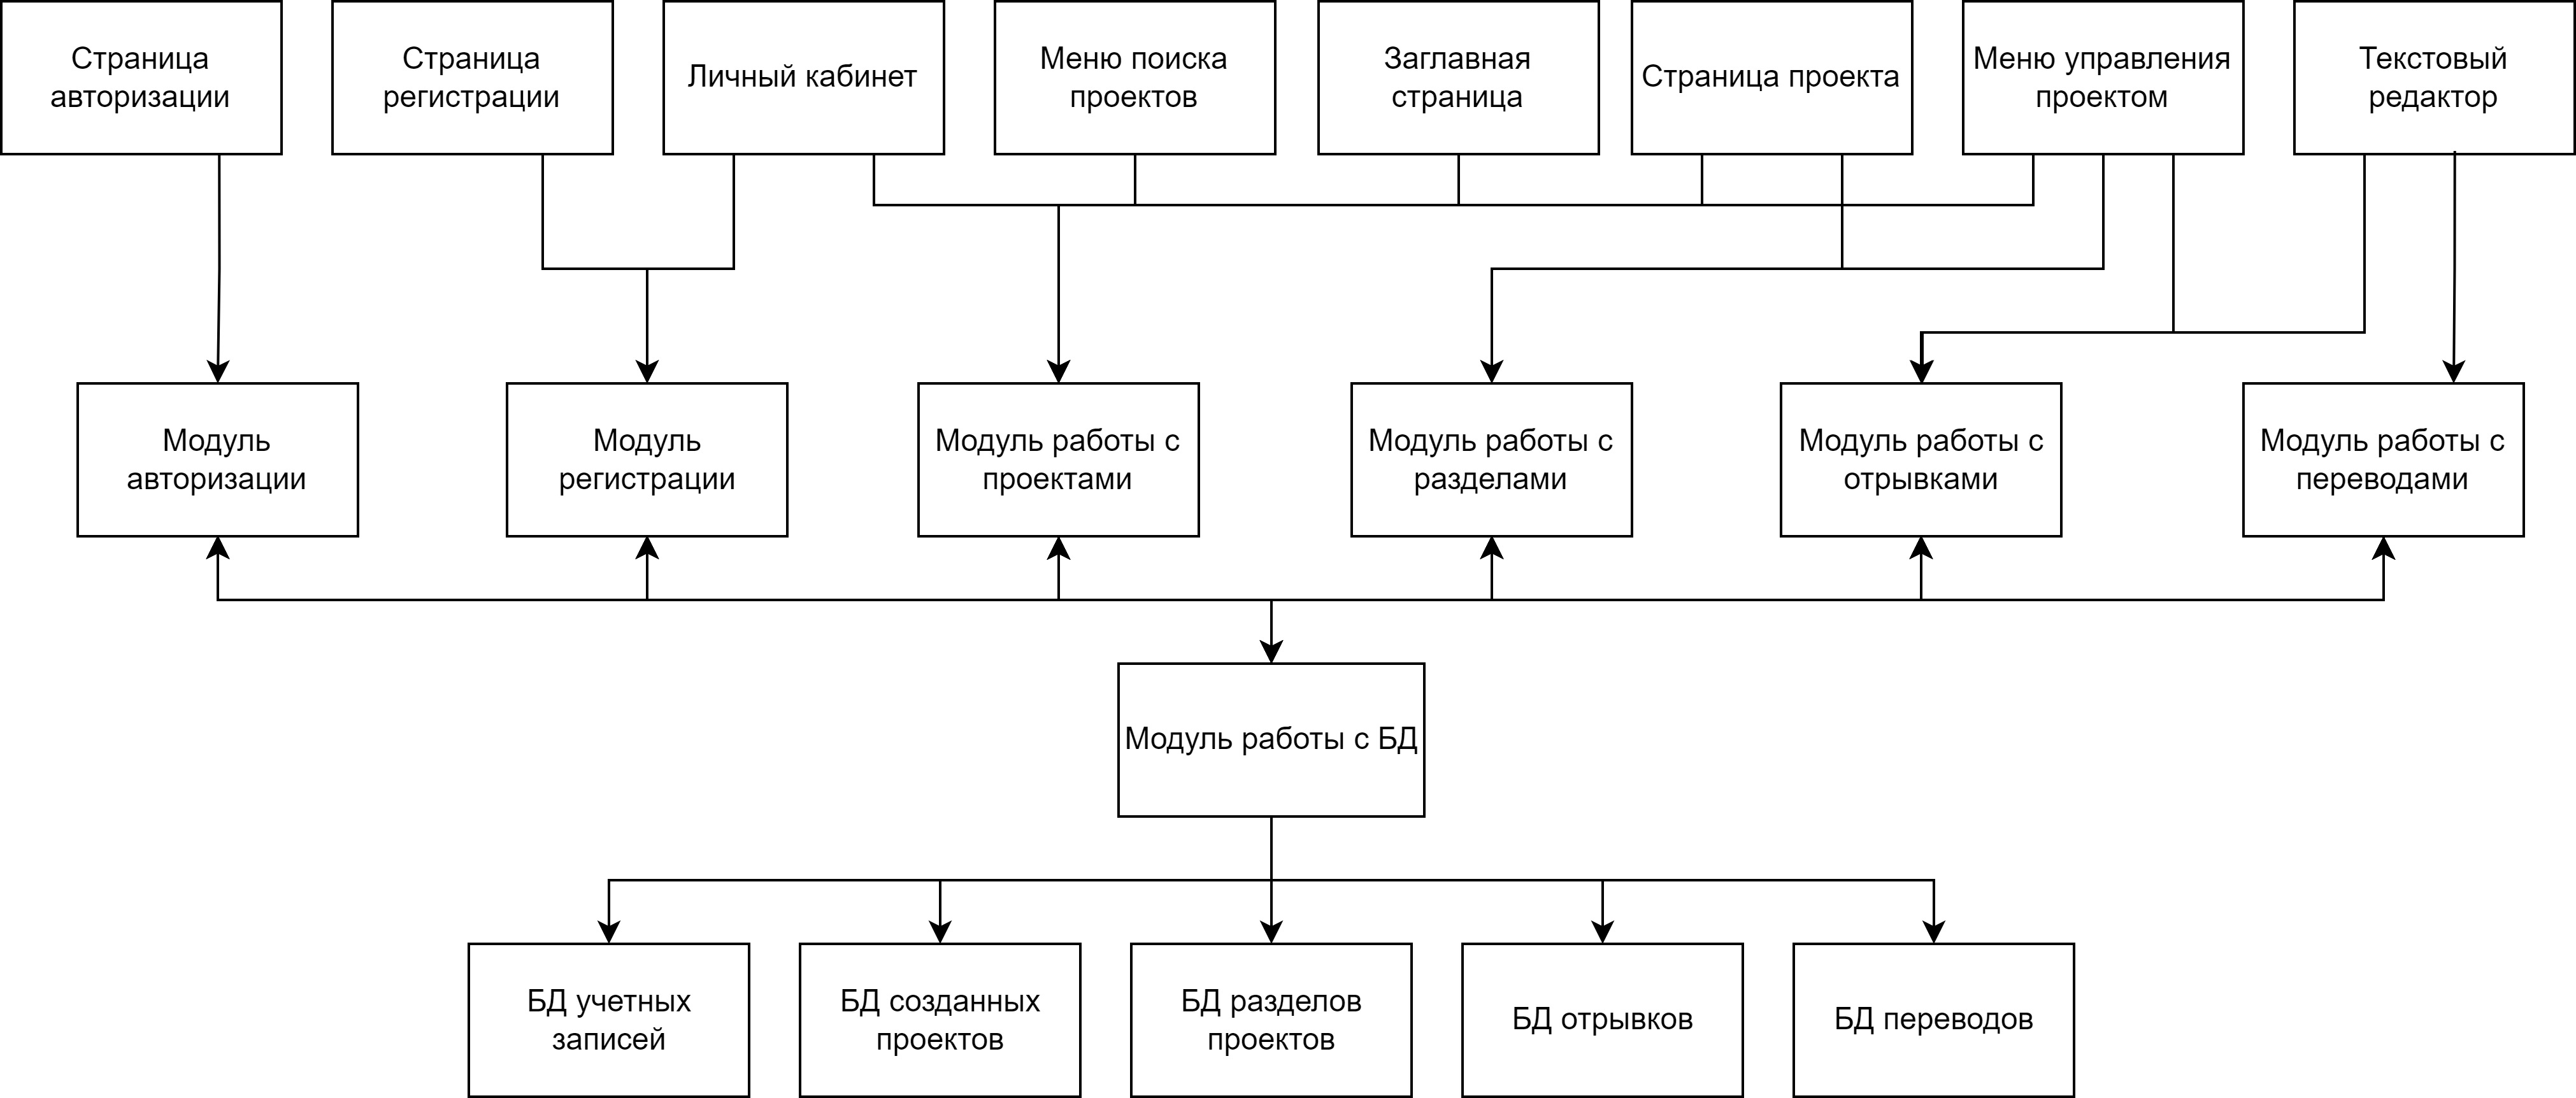
\includegraphics[width=\textwidth]{/diagrams/vaDiagram.png}
\caption{Диаграмма высокоуровневой архитектуры.}
\label{fig:diagramarchitecture}
\end{figure}




\subsection{Вывод главы}
После подробного анализа требований к разрабатываемому сервису необходимо улучшить проекты веб-страниц и реализовать клиентскую часть в соответствии с требованиями и моделями предметной области. Также необходимо спроектировать и реализовать текстовый редактор, который не был спроектирован прежде.


%%% Глава 1           %%%
%%%                   %%%
%%%%%%%%%%%%%%%%%%%%%%%%%



%%%%%%%%%%%%%%%%%%%%%%%%%
%%%                   %%%
%%% Глава 2           %%%

\newpage
\section{Описание инструментов и технологий}
\subsection{Выбор инструментов для реализации клиентской части}
HTML (HyperText Markup Language) — язык разметки, используемый для структурирования и отображения веб-страницы и ее контента. Например, контент может быть структурирован внутри множества параграфов, маркированных списков или с использованием изображений и таблиц данных. HTML не является языком программирования, и используется для того, чтобы сообщить браузеру, как необходимо отображать открытую веб-страницу. HTML-разметка позволяет создавать сколько угодно простые или сложные дизайны пользовательских интерфейсов для любых веб-сайтов. \cite{website:html}\\

CSS (Cascading Style Sheets) — язык таблицы стилей, используемый для применения стилей к элементам в документах HTML. CSS позволяет применять стили к элементам выборочно, используя классы, теги, идентификаторы и так далее. \cite{website:css}\\

Для реализации клиентской части можно использовать несколько доступных инструментов.
\subsubsection{HTML+JavaScript без использования фреймворков}
Преимущества:
\begin{itemize}
	\item[+] нет необходимости в изучении дополнительных фреймворков;
	\item[+] большая свобода в реализации, поскольку нет ограничений в виде возможностей фреймворка.
\end{itemize}

Недостатки:
\begin{itemize}
	\item[-] низкая скорость реализации;
	\item[-] значительная трудность реализации;
	\item[-] более низкое качество итогового продукта в силу отсутствия опыта разработки.
\end{itemize}

Вывод: реализация клиентской части сервиса без использования фреймворков позволит начать разработку без изучения соответствующих инструментов, однако сам этап разработки займет больше времени и усилий, будет труднее в дальнейшем поддержании кода, а итоговый продукт будет ниже качеством, поскольку реализуется неопытными разработчиками.\\



\subsubsection{React}
React — JavaScript-библиотека для разработки пользовательских интерфейсов. Основана на использовании индивидуальных компонентов, языке разметки JSX. Компонент — независимый модуль исходного кода, предназначенный для повторного использования.
Преимущества:
\begin{itemize}
	\item[+] низкий порог вхождения;
	\item[+] компонентно-ориентированная библиотека с большой базой готовых компонентов;
	\item[+] рендеринг на стороне сервера, а не клиента;
	\item[+] нисходящий поток данных;
	\item[+] виртуальная бъектная модель документа.
\end{itemize}

Недостатки:
\begin{itemize}
	\item[-] необходимо перевести HTML разметку в JSX разметку;
	\item[-] плохая документация;
	\item[-] front-end библиотека, отвечающая только за представление, т. е. back-end должен быть реализован с помощью другого инструмента.
\end{itemize}

Вывод: реализация клиентской части сервиса с помощью React будет быстрой, однако возникнет сложность при переводе HTML-шаблонов в JSX-разметку, а back-end разработка должна будет произведена с помощью другого инструмента.\\



\subsubsection{Vue.js}

Vue.js — JavaScript фреймворк, который легко надстраивается над существующим HTML и JavaScript кодом. Хорошо подходит для создания адаптируемых пользовательских интерфейсов и сложных одностраничных приложений.
Преимущества:
\begin{itemize}
	\item[+] позволяет оптимизировать HTML-разметку с помощью компонентов;
	\item[+] легкая интеграция в существующую инфраструктуру;
	\item[+] легкость в масштабировании;
	\item[+] малый размер самого фреймворка.
\end{itemize}

Недостатки:
\begin{itemize}
	\item[-] нехватка документации на английском языке;
	\item[-] нехватка ресурсов — очень малый процент разработчиков используют Vue.js для крупных проектов;
	\item[-] проблемы при интеграции в большие проекты, при этом отсутствует опыт возможных решений подобной проблемы.
\end{itemize}

Вывод: Vue.js в силу своего небольшого размера позволяет быстро реализовать сложное одностраничное приложение или улучшить существующий проект, однако имеет очень маленькую аудиторию и недостаточную документацию на английском языке (фреймворк разработан китайскими компаниями), что повышает вероятность появления тяжело разрешаемых проблем при масштабировании.\\



\subsubsection{Vue.js}

Angular — платформа для разработки веб-приложений, основанная на языке TypeScript.
Преимущества:
\begin{itemize}
	\item[+] очень подробная документация;
	\item[+] двусторонняя привазка данных — минимальный риск ошибок приложения;
	\item[+] ускоренная компиляция;
	\item[+] модель Model-View-ViewModel, пользованяющая разработчикам раздельно работать в одном разделе приложения с использованием одного и того же набора данных.
\end{itemize}

Недостатки:
\begin{itemize}
	\item[-] необходимость изучения сложного синтаксиса TypeScript;
	\item[-] проблемы с миграцией при переходе между версиями фреймворка — поддерживать приложение на протяжении многих лет будет проблематично.
\end{itemize}

Вывод: Angular является очень популярной и эффективной платформой, однако требует изучения TypeScript, что значительно замедлит процесс разработки, поскольку уже реализованные шаблоны и веб-API станут непригодны для разработки.\\

\subsection{Вывод}
Исходя из преимуществ и недостатков рассмотренных инструментов, библиотек и фреймворков, было принято решение использовать React.js, поскольку эта библиотека на данный момент является наиболее популярной, то есть имеет низкий порог вхождения и подробную документацию, что значительно ускорит процесс разработки. Помимо этого React.js поддерживает Bootstrap в виде библиотеки компонент React Bootstrap, что позволит легко и быстро адаптировать уже существующие шаблоны для разработки клиентской части. Ориентированность React на front-end составляющую не является существенным недостатком для этого проекта, поскольку back-end разработка проводится с помощью платформы Node.js и будет легко интегрирована с front-end составляющей с помощтю веб-API.\\


%%% Глава 2           %%%
%%%                   %%%
%%%%%%%%%%%%%%%%%%%%%%%%%



%%%%%%%%%%%%%%%%%%%%%%%%%
%%%                   %%%
%%% Глава 3           %%%

\newpage
\section{Разработка клиентской части приложения}

Листинги кода front-end составляющей доступны по ссылке:\\
\href{https://github.com/ipaingo/Desman-Translate-frontend}{https://github.com/ipaingo/Desman-Translate-frontend}\\

Для разработки клиентской части было необходимо выполнить несколько этапов.

\subsection{Улучшение и перевод существующих HTML-шаблонов}
Поскольку React.js использует язык разметки JSX, а React Bootstrap, который крайне удобно использовать вместе с React.js предлагает не библиотеку CSS-файлов, а готовых React-компонентов, было необходимо перевести HTML-шаблоны в JSX-разметку. Для перевода между языками разметок использовались онлайн-инструменты, преобразование полученных блоков разметки для использования с React Bootstrap было выполнено вручную, поскольку являлось простой и быстрой в выполнении задачей.

\begin{figure}[H]
\centering
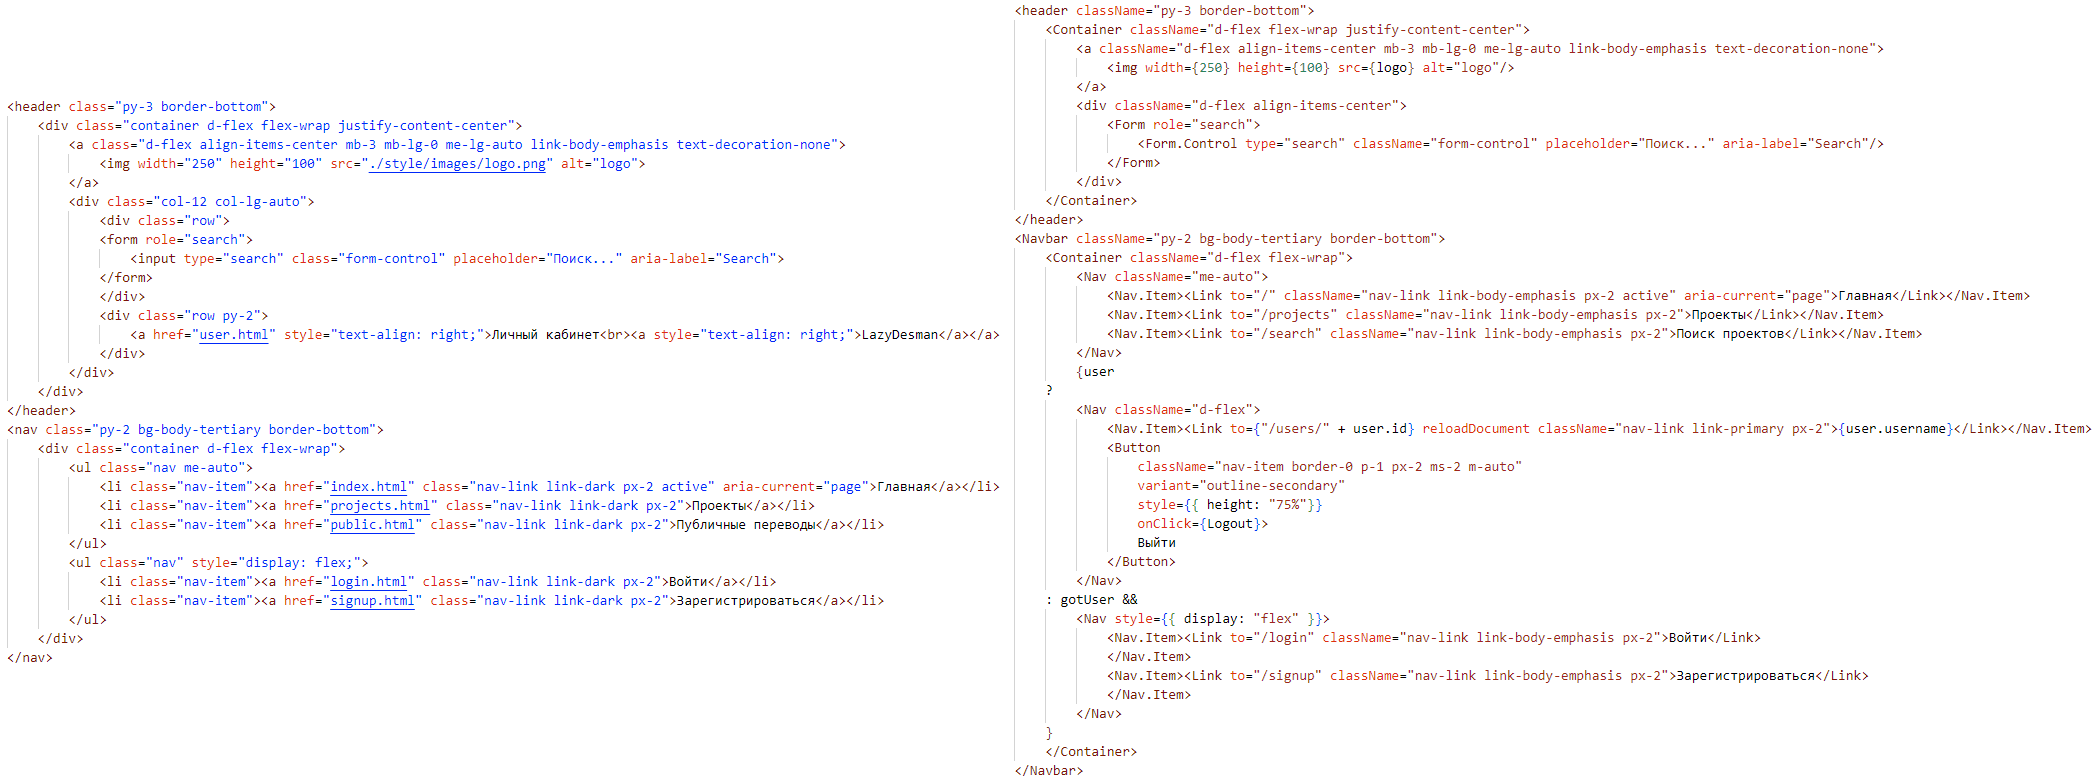
\includegraphics[width=\textwidth]{/diagrams/newCode.png}
\caption{Пример изменения разметки после перевода.}
\label{fig:diagramnewcode}
\end{figure}

\subsection{Установка React.js}
Для разработки с помощью React.js необходимо установить его локально на свой рабочий компьютер. Установка готового приложения на сервер является частью back-end разработки проекта, поэтому не будет рассмотрена в этой работе.

\begin{enumerate}
\item Установить Node.js на рабочий компьютер.
\item Открыть терминал командной строки в директории, где должен быть установлен React.
\item Ввести команду \texttt{npm install react react-dom}.
\item При необходимости использовать некоторую библиотеку для работы с React необходимо в терминале ввести команду \texttt{npm install <название библиотеки>}.
\end{enumerate}

Установщик npm формирует файл зависимостей, поэтому при установке готового проекта на React на другой рабочий компьютер необходимо в терминале выполнить команду \texttt{npm install}. Тогда все необходимые библиотеки будут установлены автоматически в соответствии с файлом зависимостей.

\subsection{Запросы к API и отрисовка страницы в зависимости от ответа}
Для взаимодействия с API были реализованы несколько функций, совершающих fetch-запросы и возвращающих ответы в зависимости от введенных параметров.


\begin{lstlisting}[language=JavaScript, caption={Вспомогательная функция, использующаяся для осуществления fetch-запросов с параметрами.}]
export async function fetchSomeAPI(link, method = "GET", body = {}) {
    let options = { method: method, }
    if (method == 'POST' || method == 'PATCH') {
        options.body = JSON.stringify(body)
        options.headers = { 'Content-Type': 'application/json; charset=UTF-8', }
    }

    const response = await fetch(link, options)
    if (!response.ok) {
        throw { status: response.status, errors: JSON.parse(await response.text() || "{}")?.errors }
    }
    try {
        let data = await response.json()
        return data
    } catch (err) {

    }
}
\end{lstlisting}

Для аутентификации пользователя используется компонент AuthProvider, функция ReAuth которого совершает запрос к API с попыткой получить пользователя, возвращает информацию о том, что пользователь не прошел аутентификацию, если проверка была неуспешной, возвращает информацию о пользователе в случае успеха.


\begin{lstlisting}[language=JavaScript, caption={Компонент AuthProvider, необходимый для аутентификации пользователя.}]
function AuthProvider(props) {
    const [user, setUser] = useState(undefined);
    const [gotUser, setGotUser] = useState(false);

    async function ReAuth() {
        console.log("okay, try to get me")
        let rsp = await fetch("/api/whoami",
        {
            method: "GET",
            headers: {
                'Content-Type': 'application/json; charset=UTF-8',
            },
        })
        console.log(rsp)
        if (!rsp.ok) {
            console.log("what")
            setUser(undefined)
            return
        }

        try {
            rsp = await rsp.json()
            console.log("user")
            console.log(rsp)
        } catch (err) {
            rsp = null
            console.log("no user :(")
        }

        setUser(rsp)
    }

    const value = {
        user,
        ReAuth,
        gotUser,
    };


    useEffect(() => {
        ReAuth();
    }, [])

    useEffect(() => {
        setGotUser(user !== undefined)
    }, [user])

    return <AuthContext.Provider value={value} {...props} />;
}
\end{lstlisting}

Функции с fetch-запросами вызываются в коде для получения необходимой для отрисовки информации.


\begin{lstlisting}[language=JavaScript, caption={Код на JavaScript, получающий необходимую информацию для отрисовки главной страницы.}]
function Home() {

    const { user } = useContext(AuthContext);

    const [recentProjects, setRecentProjects] = useState([]);

    const [popularProjects, setPopularProjects] = useState([]);

    async function GetRecentProjects() {
        if (!user)
            return

        try {
            let projects = (await fetchUser(user.id, true)).projects
            projects.sort((a, b) => new Date(b.created_at) - new Date(a.created_at))
            setRecentProjects(projects)
        } catch (err) {
            console.log(err)
        }
    }


    async function GetPopularProjects() {
        try {
            let projects = await fetchProjects(4)
            projects.sort((a, b) => new Date(b.created_at) - new Date(a.created_at))
            setPopularProjects(projects)
        } catch (err) {
            console.log(err)
        }
    }


    useEffect(() => {
        GetRecentProjects();
    }, [user]);

    useEffect(() => {
        GetPopularProjects();
    }, []);


    let navigate = useNavigate();
    const routeChange = () => {
        let path = '/create';
        navigate(path);
    }
<...>
\end{lstlisting}

React Bootsrap предоставляет разработчику большую библиотеку готовых компонент, которые были использованы при написании кода. Далее приведен пример JSX-разметки со вставками кода на JavaScript, отрисовывающий главную страницу веб-сайта.

\begin{lstlisting}[language=HTML, caption={Код на JSX, отрисовывающий главную страницу.}]
<Header />
<Container className="mt-5">
    <Row>
        <Col sm={6} className="text-left pe-5">
            <h2 className="mb-4">Recent projects:</h2>
            {recentProjects.map((project, i) =>
                <Container className="text-left pb-2" key={project.id}>
                    <Stack direction="horizontal" gap="10" className="border rounded p-3 mt-1">
                        <img
                            width={60}
                            height={60}
                            src={placeholder}
                            alt="thumbnail"
                        />
                        <Container className="text-left text-break">
                            <Link to={"/projects/" + project.handle} className="link-primary">
                                {project.name}
                            </Link>
                            <br /> {project.description}
                        </Container>
                    </Stack>
                </Container>
            )}

            <h2 className="my-4">Trending projects:</h2>
            {popularProjects.map((project, i) =>
                <Container className="text-left pb-2" key={project.id}>
                    <Stack direction="horizontal" gap="10" className="border rounded p-3 mt-1">
                        <img
                            width={60}
                            height={60}
                            src={placeholder}
                            alt="thumbnail"/>
                        <Container className="text-left text-break">
                            <Link to={"/projects/" + project.handle} className="link-primary">
                                {project.name}
                            </Link>
                            <br /> {project.description}
                        </Container>
                    </Stack>
                </Container>
            )}


        </Col>
        <Col className="border-top border-start rounded py-1 mt-3 ps-3">
            <h5 className="py-2 border-bottom" >
                What is Desman Translate?
            </h5>
            <p>
                <...>
            </p>
            <h5 className="py-2 border-bottom">
                How does this work?
            </h5>
            <p>
                <...>
            </p>
            <p>
                <...>
            </p>
            <p>Have a lot of fun...</p>
            {user && 
                <Button variant="primary"
                    onClick={routeChange}>
                    Create a project
                </Button>
            }
        </Col>
    </Row>
</Container>
<Footer />
\end{lstlisting}

Результат работы кода, описанного выше:

\begin{figure}[H]
\centering
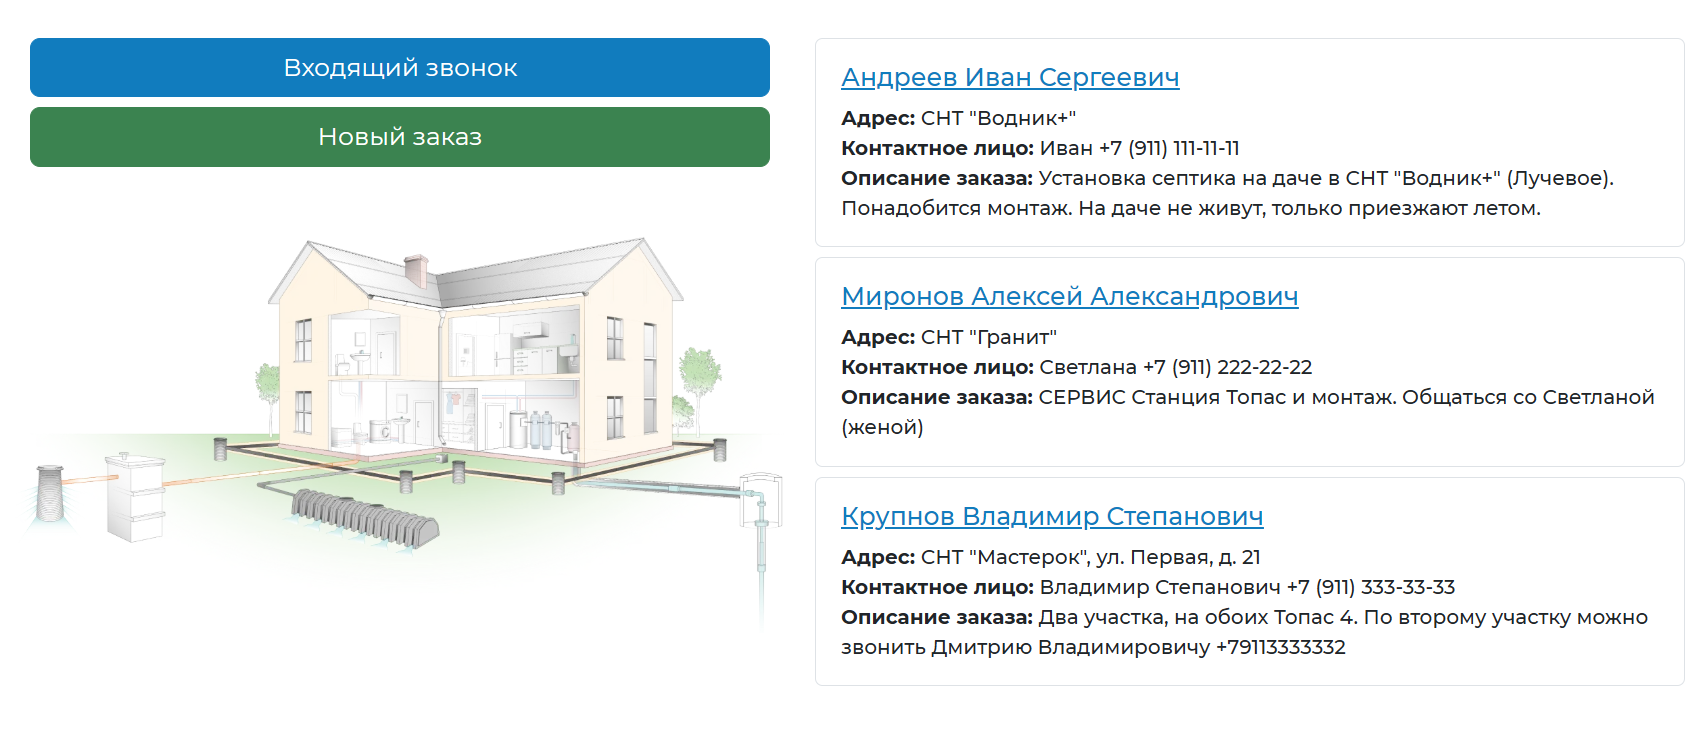
\includegraphics[width=\textwidth]{/manual/home.png}
\caption{Главная страница сайта.}
\label{fig:pagehome}
\end{figure}

\subsection{Сборка и установка сервиса}

\subsubsection{Установка сервера}
\begin{enumerate}
\item Перейти по ссылке на страницу репозитория на сайте GitHub.com: https://github.com/Neprim/DesmanTranslateBackend.
\item Установить базу данных MongoD: https://www.mongodb.com/try/download/community.
\item Скачать и разархивировать проект или клонировать git-репозиторий на сервере или в локальном хранилище.
\item Настроить конфигурационный файл .env: \verb|JWT_SECRET| - параметр для шифровки cookie-файлов.
\item Открыть терминал, перейти в папку скачанного проекта, убедиться, что пользователь имеет установщик пакетов npm и node. Выполнить команду \verb|npm install|.
\item В терминале выполнить команду \verb|node index.js| - сервер запущен.
\end{enumerate}

\subsubsection{Установка клиента}
\begin{enumerate}
\item Перейти по ссылке на страницу репозитория в GutHub.com: https://github.com/ipaingo/Desman-Translate-frontend.
\item Скачать и разархивировать проект или клонировать git-репозиторий на сервере или в локальном хранилище.
\item Открыть терминал, перейти в папку скачанного проекта, убедиться, что пользователь имеет установщик пакетов npm и node. Выполнить команду \verb|npm install|.
\item Если необходимо запустить сайт на локальном сервере – написать команду в терминале \verb|npm start|. Сайт будет доступен по адресу \verb|http://localhost:3000/|
\item Если необходимо развернуть сайт на сервере – написать команду \verb|npm run build|. Создастся директория \verb|build| – это готовое приложение, которое можно разместить на сервере.
\end{enumerate}
%%% Глава 3           %%%
%%%                   %%%
%%%%%%%%%%%%%%%%%%%%%%%%%



%%%%%%%%%%%%%%%%%%%%%%%%%
%%%                   %%%
%%% Заключение        %%%

\newpage
\section*{Заключение}
\addcontentsline{toc}{section}{Заключение}


%%% Заключение        %%%
%%%                   %%%
%%%%%%%%%%%%%%%%%%%%%%%%%



%%%%%%%%%%%%%%%%%%%%%%%%%
%%%                   %%%
%%% Литература        %%%

\newpage
\addcontentsline{toc}{section}{Список литературы}
\bibliographystyle{plain}
\bibliography{refs}

%%%  Литература       %%%
%%%                   %%%
%%%%%%%%%%%%%%%%%%%%%%%%%



%%%%%%%%%%%%%%%%%%%%%%%%%
%%%                   %%%
%%% Приложение        %%%

\newpage
\section*{Приложение}
\addcontentsline{toc}{section}{Приложение}



%%% Приложение        %%%
%%%                   %%%
%%%%%%%%%%%%%%%%%%%%%%%%%
 

\end{document}